
\documentclass[12pt,article]{memoir}

\usepackage{fancyhdr}
\usepackage{graphicx}
\usepackage{fontspec}
\setmainfont{Calibri}
\usepackage{tikz}
\usetikzlibrary{calc}
\usepackage{xcolor}
\usepackage{xpatch}
\usepackage{hyperref}

\usepackage{fancyhdr}
\usepackage{graphicx}
\usepackage{fontspec}
\setmainfont{Calibri}
\usepackage{tikz}
\usetikzlibrary{calc}
\usepackage{xcolor}
\usepackage{xpatch}
\usepackage{hyperref}
\usepackage{tabu}
\usepackage{float}
\usepackage[autostyle, english = american]{csquotes}


\usepackage[yyyymmdd]{datetime} % change date format to yyyy/mm/dd to fit ISO8601

\renewcommand{\familydefault}{\sfdefault} % set font
\renewcommand{\dateseparator}{--} % change date-seperators to - to fit ISO8601

\renewcommand\contentsname{Table of Contents}

\chapterstyle{section}
\renewcommand*{\chapnumfont}{\normalfont\HUGE\bfseries\sffamily}
\renewcommand*{\chaptitlefont}{\normalfont\HUGE\bfseries\sffamily}

\makeatletter 
% define macro for itemcode
\newcommand\itemcode[1]{\renewcommand\@itemcode{#1}}
\newcommand\@itemcode{}

% define macro for rev number
\newcommand\revnumber[1]{\renewcommand\@revnumber{#1}}
\newcommand\@revnumber{}
\makeatother

\definecolor{orbitOrange}{RGB}{250,62,0} % the ORBiT orange

\setlrmarginsandblock{2.5cm}{2.5cm}{*}
\setulmarginsandblock{2.5cm}{*}{1}
\checkandfixthelayout 

\setlength{\beforechapskip}{0cm} % reduce chapter spacing

\hypersetup{
    colorlinks,
    citecolor=black,
    filecolor=black,
    linkcolor=black,
    urlcolor=black
}

%**********************************************************************
%Document titles etc. defined here: (replace [] as well)
\title{ORBiT Avionics System II Requirements}
\author{Jinzhi Cai}
\itemcode{ES00002}
\revnumber{A03}
\date{\today}
%end of document titles etc.
%**********************************************************************

\makeatletter
\let\runtitle\@title
\let\runitemcode\@itemcode
\makeatother

% set header style
\pagestyle{fancy}
{
	\fancyheadoffset{0cm}

	\lhead{\runtitle \ - \runitemcode}
	\rhead{Page: \thepage }
	%\chead{\leftmark} % section name
}

\newcommand{\OrbitBackground}{% For a logo drawn with TikZ
\begin{tikzpicture}[remember picture,overlay] % draw background
	\coordinate (bl) at (current page.south west);
	\coordinate (r) at (current page.east);
    \coordinate (A) at ($(bl)+(0,3cm)$);
    \coordinate (B) at ($(r)+(0,-2cm)$);
    \coordinate (C) at (current page.south east);
    \coordinate (ctrlNode) at ($(current page.south) + (0cm,1cm)$);
    \coordinate (ctrlNode2) at ($(current page.south east) + (-1cm,1cm)$);
    \fill[orbitOrange, fill opacity=0.2]
    (A) .. controls (ctrlNode) and (ctrlNode2) .. (B) -- (C) -- (bl);
    \node [white] at ($(C) + (-3cm,1cm)$) {2015-\the\year \ ORBiT@SU};
\end{tikzpicture}
}

\cfoot{\OrbitBackground}

\begin{document}

\begin{tikzpicture}[remember picture,overlay] % draw background
	\coordinate (bl) at (current page.south west);
	\coordinate (r) at (current page.east);
    \coordinate (A) at ($(bl)+(0,3cm)$);
    \coordinate (B) at ($(r)+(0,-2cm)$);
    \coordinate (C) at (current page.south east);
    \coordinate (ctrlNode) at ($(current page.south) + (0cm,1cm)$);
    \coordinate (ctrlNode2) at ($(current page.south east) + (-1cm,1cm)$);
    \fill[orbitOrange]
    (A) .. controls (ctrlNode) and (ctrlNode2) .. (B) -- (C) -- (bl);
    \node [white] at ($(C) + (-3cm,1cm)$) {2015-\the\year \ ORBiT@SU};
\end{tikzpicture}

\makeatletter
	
\includegraphics[width=\textwidth]{../logo.jpg}\\[4ex]
	\begin{center}
	{\fontsize{50}{60}\selectfont \bfseries  \@title }\\[2ex] 
	{\LARGE  \@itemcode}\\
	\end{center}
	\begin{flushright}
	\vspace*{\fill}
	{\LARGE Rev: \@revnumber}\\[2ex]
	{\large \@author}\\[2ex]
	{\large \@date}\\[20ex]
	\end{flushright}
\makeatother
\thispagestyle{empty}
\newpage

\tableofcontents*
\thispagestyle{fancy}
\newpage

%**********************************************************************
% Everything after this is the main document. Edit below this line,

\chapter{System Description}
\section{Introduction}
The ORBiT Avionics System II (OA-II) is the next generation avionics system for the Orange Rocket Ballistics Team experimental hybrid rocket. It include two major assemblies, the Vehicle Electronics, and the Base Station Electronics. All components in the OA-II system are interconnected with a unique backplane system and wireless system.\\
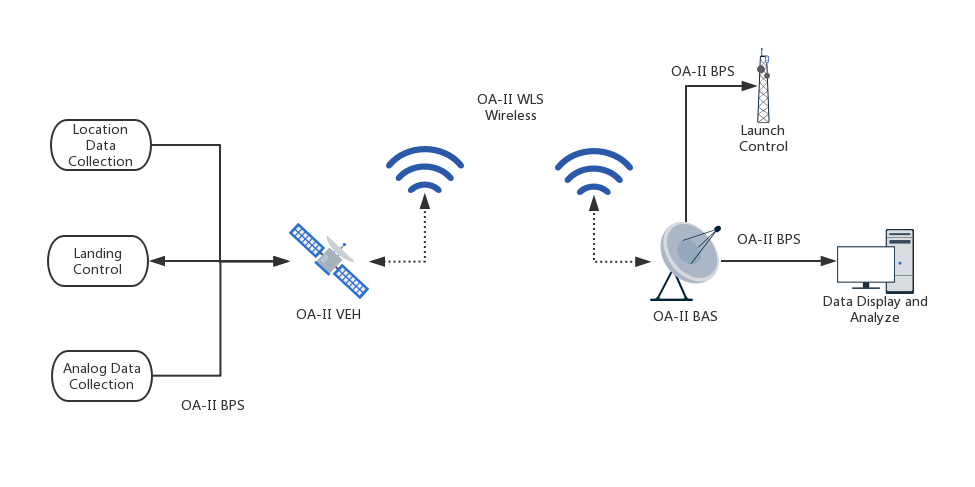
\includegraphics[width=\textwidth]{sys_diag.png}
\subsection{Vehicle Electronics (VEH)}
The OA-II VEH is used to control the rocket's various subsystems, collect information about the rocket's performance, and communicate this with the BAS for remote control and monitoring. It also has autonomous software and onboard storage, to allow for continued operation in case of failure of the wireless link.
\subsection{Base Station Electronics (BAS)}
The OA-II BAS is used to communicate wirelessly with the VEH and perform basic realtime analysis on rocket status. The BAS provides live location and performance information, and data storage for further analysis. The BAS can also help to locate the rocket after landing.
\subsection{Engine Testing System (ETS)}
TBD
\subsection{Backplane System (BPS)}
The OA-II BPS is a unique, multi-level information exchange system that links modules in in the OA-II VEH and BAS. It provides different speed modes for different components.
\subsection{Wireless System (WLS)}
The OA-II WLS is a wireless communication system which provides communication between the VEH and BAS. It also provides a basic location landing signal in case of failure of other subsystems.
\section{Requirement}
\subsection{Vehicle Electronics (VEH)}
\begin{itemize}
\item Data receiving and transmission to base station
\item 3D linear kinematics data.
\begin{itemize}
	\item $X$, $Y$, $Z$ (position)
	\item $V_X$, $V_Y$, $V_Z$ (velocity)
	\item $A_X$, $A_Y$, $A_Z$ (acceleration)
\end{itemize}
\item 3D rotational kinematics data
\begin{itemize}
	\item $\theta_X$, $\theta_Y$, $\theta_Z$ (position)
	\item $\omega_X$, $\omega_Y$, $\omega_Z$ (velocity)
	\item $\alpha_X$, $\alpha_Y$, $\alpha_Z$ (acceleration)
\end{itemize}
\item Static and dynamic air pressure
\item Redundant 28V power supplies and power management
\item High frequency data collection ($F_s \geq 10kHz$)
\item Actuator and ignitor control ($P_{pk} \geq 50W$)
\item 1080p 60Hz RGB Camera $\times$ 4
\item Landing location broadcast (up to 2 hours, 3km range, low power consumption)
\end{itemize}
\subsection{Base Station Electronics (BAS)}
\begin{itemize}
\item Data receiving and transmission to rocket
\item Display rocket status information 
\item Basic data analysis (normal/warning/error status).
\item Live location display
\item Ignition control system
\item Engine oxidizer control system
\item Safety oxidizer cutoff
\item Parachute control
\item Launch control
\item Automatic system checking
\end{itemize}
\subsection{Engine Testing System (ETS)}
\begin{itemize}
\item TBD
\end{itemize}
\subsection{Backplane System (BPS)}
\begin{itemize}
\item Provide different speed modes with low latency
\begin{itemize}
\item Info level ($\leq 3MB/s$)
\item Data level ($\approx 50MB/s$)
\item Stream level ($\geq 100MB/s$)
\end{itemize}
\item Tolerate high vibration and EMI
\item Tolerate high temperature ($\leq 75^{\circ}C$)
\end{itemize}
\subsection{Wireless System (WLS)}
\begin{itemize}
\item High speed wireless link (10MB/s, 3km range)
\item Low speed wireless link (1kB/s, 10km range) with time-of-flight location
\end{itemize}
\chapter{Revision History}
\begin{table}[H]
	\centering
	\begin{tabu}{r || c | c | c }
		Rev\# & Editor & Delta & Date\\ \hline
		A01 & Jinzhi Cai & Initialize  & 2019-06-21 \\
		-	& Jinzhi Cai & Add Radio requirement & 2019-06-24 \\ \hline
		A02 & Gabriel Smolnycki & Edits for clarity & 2019-06-25\\ \hline
		A03 & JInzhi Cai & Add Engine Testing System & 2019-07-04\\ \hline
	\end{tabu}
	\caption{Summary of Revision History}
	\label{tab:edatools}
\end{table}

%end of document
%**********************************************************************
\end{document}